% Use your own class of Latex document here
\documentclass{evolang9_book}
%\usepackage[latin1]{inputenc}
%\usepackage[T1]{fontenc}
\usepackage{multicol}
\usepackage[english]{babel}
\usepackage[final]{pdfpages}
%\usepackage[margin=2cm,includehead,a5paper]{geometry}
\usepackage{makeidx}
\usepackage{index}
\usepackage[bookmarks=yes]{hyperref}
\usepackage[none]{hyphenat}
\usepackage{enumitem}
\makeindex

% Declare the index of authors. Note: the index must
% be produced with the following command (after a first Latex compilation):
% makeindex proceedings.ax -o proceedings.ad
%\newindex{authors}{ax}{ad}{Index of authors}

% Some pdfpages parameters
\includepdfset{pages=-,pagecommand={}}

\includepdfset{pages=-,pagecommand={}}
\usepackage{tocloft}
\renewcommand\cftchapfont{\fontsize{10}\bfseries}
\renewcommand\cftsecfont{\fontsize{10}}
\renewcommand\cftchappagefont{\fontsize{10}\bfseries}
\renewcommand\cftsecpagefont{\fontsize{10}}
\setlength\cftparskip{2pt}
\setlength\cftbeforechapskip{0pt}
\setlength{\footskip}{80pt}

% OK, here begins the document
\begin{document}

% The title page
\title{ \textbf{Proceedings EVOLANG 11 (New Orleans 2016)}}
\author{}
%\date{\today}

%\maketitle
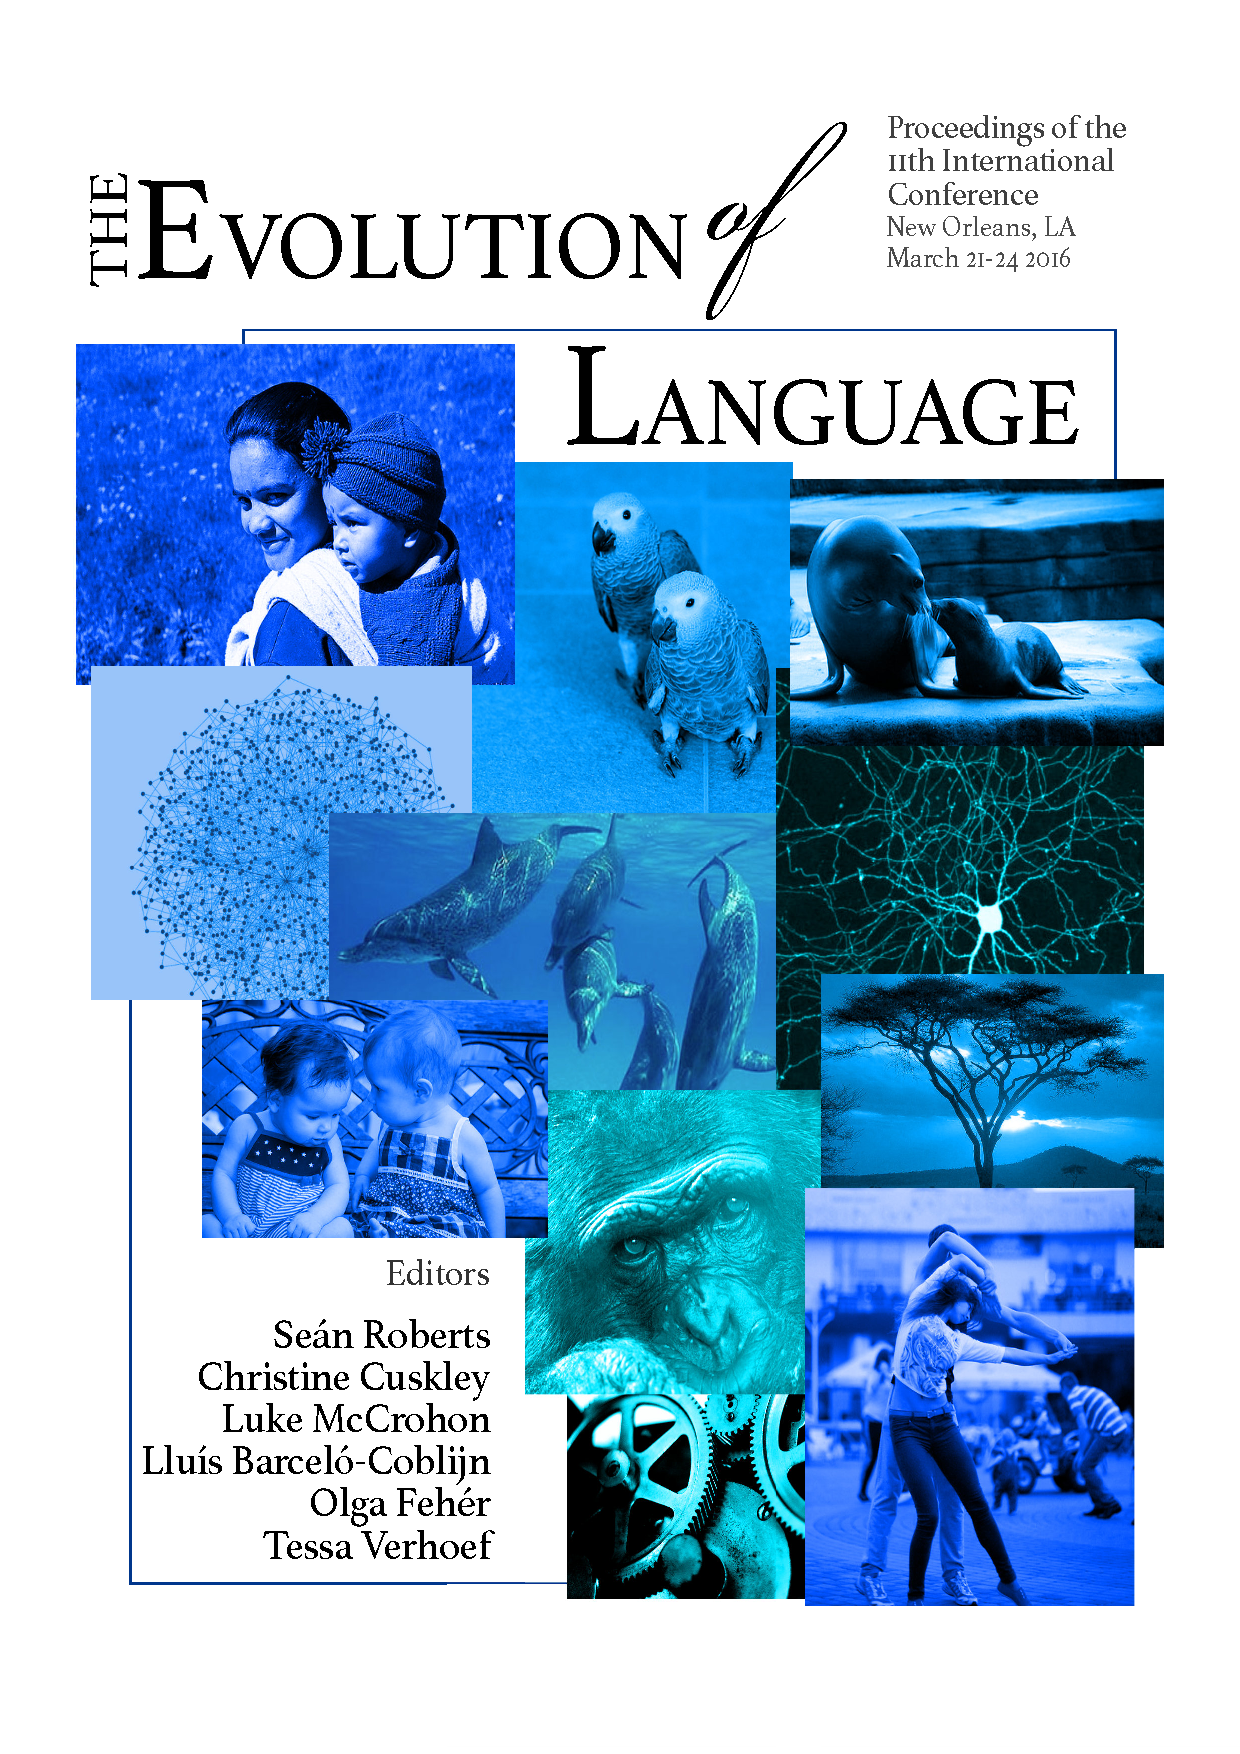
\includepdf[pages={1}]{cover/EvoLangCover.pdf}

\chapter*{}
The Evolution of Language: Proceedings of the 11th International Conference.  New Orleans, USA.
\\\\
Cover image credits:
https://www.flickr.com/photos/sjcockell/4684828794
 : Simon Cockell
\\\\
https://www.flickr.com/photos/69221340@N04/8652893210
: Papooga
\\\\
https://www.flickr.com/photos/jdebberly/2850385433
: Jay Ebberly
\\\\
https://www.flickr.com/photos/pustovit/14336071644
: Vladimir Pustovit
\\\\
https://www.flickr.com/photos/kittysfotos/10037699755
: Kitty Terwolbeck
\\\\
https://www.flickr.com/photos/ajmat/3730694413
: AJ.Mat
\\\\
https://www.flickr.com/photos/neilspicys/2348972925
: NeilsPhotography
\\\\
https://www.flickr.com/photos/kapten/1085243998
: Bj\"{o}rn S\"{o}derqvist
\\\\
https://www.flickr.com/photos/thomasclaveirole/463202335
: Thomas Claveirole
\\\\
https://www.flickr.com/photos/deanwissing/3565255880
: Dean Wissing
\\\\
https://www.flickr.com/photos/mikeblogs/3101400087
: Mike Seyfang

% Foreword: add your own text
\chapter*{Preface}
\addcontentsline{toc}{chapter}{Preface}
{%Preface
This volume collects the refereed papers and abstracts of the 11th International Conference on the Evolution of Language (EVOLANG XI), held in New Orleans on 21st-24th March, 2016.  Submissions to the conference were solicited in two forms, papers and abstracts, and this is reflected in the structure of this volume.
\\
The biennial EVOLANG conference is characterised by an invigorating, multi-disciplinary approach to the origins and evolution of human language, and brings together researchers from many fields including anthropology, archaeology, artificial life, biology, cognitive science, computer science, ethology, genetics, linguistics, neuroscience, palaeontology, primatology, psychology and statistical physics.  The multi-disciplinary nature of the field makes the refereeing process for EVOLANG very challenging, and we are indebted to our panel of reviewers for their very conscientious and valuable efforts.
\\
For the first time, the proceedings of EvoLang XI are primarily available online in an open access format.  Please visit \url{http://evolang.org/neworleans/} for up-to-date papers, workshop papers and supplementary materials.  Thanks are due to the following people:\\\\
%
\textbf{The EVOLANG committee:}
    \begin{itemize}
\item Andreas Baumann (University of Vienna),
\item    Rudolf Botha (Stellenbosch University),
\item    Christine Cuskley (Institute for Scientific Interchange),
\item    Erica Cartmill (University of California, Los Angeles) [First Contact/Co-chair],
\item    Jean-Louis Dessalles (Ecole Nationale Sup�rieure des T\`{e}l\`{e}communications, Paris),
\item    Ramon Ferrer i Cancho (Polytechnic University of Barcelona),
\item    Tecumseh Fitch (University of Vienna),
\item    Jim Hurford (University of Edinburgh),
\item    Simon Kirby (University of Edinburgh) [Co-chair],
\item    Chris Knight (University of East London),
\item    Heidi Lyn (University of Southern Mississippi),
\item    Luke McCrohon (University of Tokyo) [Webmaster],
\item    Kazuo Okanoya (University of Tokyo),
\item    Thom Scott-Phillips (Durham University),
\item    Andrea Ravignani (University of Vienna, University of Edinburgh),
\item    Nikolaus Ritt (University of Vienna),
\item    Kenny Smith (University of Edinburgh) [Treasurer],
\item    Maggie Tallerman (Newcastle University, UK),
\item    Natalie Uomini (University of Liverpool).
\end{itemize}
%
\textbf{The local organising committee:}\\
 University of Southern Mississippi:
 Heidi Lyn (Chair),
 Megan Broadway,
    Mystera Samuelson,
    Jennie Christopher,
 and  Beatrice Chenkin.  \\
University of South Alabama:  Stephanie Jett.\\
Tulane University: Olanike-Ola Orie.  \\
Louisiana State University: XiaoChing Li\\\\
%
%
%
\textbf{The workshop convenors:}
Christine Cuskley, Vittorio Loreto, Francesca Tria, Vito D.P. Servedio, Andrea Ravignani, Erin E. Hannon, Se\'{a}n Roberts, Gregory J. Mills, Madza Farias-Virgens, Dillon Niederhut, Terrence Deacon, Tecumseh Fitch, Bart de Boer and Takeshi Nishimura.\\\\
%
%
\textbf{The plenary speakers:}
Sharon Thompson-Schill, Thom Scott-Phillips, Ljiljana Progovac, Richard Moore, Erich Jarvis, Vincent Janik, Evelina Fedorenko, Dean Falk, Joan Bybee.
%
\\\\
Finally, and most importantly, the authors of all the contributions collected here.
%
\begin{flushright}Se\'{a}n Roberts, Christine Cuskley, Luke McCrohon,\\ Llu\'{i}s Barcel\'{o}-Coblijn, Olga Feher and Tessa Verhoef.
\\ Scientific Committee,
\\February 2016\end{flushright}
}  % End preface
\newpage

\chapter*{Reviewers}
\begin{multicols}{3}
\begin{itemize}[label={},leftmargin=*]
\item Alan Nielsen
\item Albert Naccache
\item Aleksandrs Berdicevskis
\item Alex Carstensen
\item Alfredo Ardila
\item Andrea Ravignani
\item Andreas Baumann
\item Andreea Geambasu
\item Andrew Feeney
\item Andrew Wedel
\item Anne Marie Di Sciullo
\item Anne van der Kant
\item Anneliese Kuhle
\item Antoni Gomila
\item Antonio Ben\'{i}tez-Burraco
\item Aritz Irurtzun
\item Ashley Micklos
\item Barbora Skarabela
\item Bart de Boer
\item Bill Thompson
\item Bodo Winter
\item Brady Clark
\item Camilla Power
\item Carel ten Cate
\item Carl Vogel
\item Carlos Santana
\item Carmen Saldana
\item Catriona Silvey
\item Cedric Boeckx
\item Chris Knight
\item Christian Abry
\item Christina Behme
\item Christine Caldwell
\item Christine Cuskley
\item Connie de Vos
\item Cory M Cuthbertson
\item Damian Blasi
\item Dan Dediu
\item Daniel Dor
\item Daniel Lenzen
\item Dankmar Enke
\item David Leavens
\item David Lightfoot
\item Dillon Niederhut
\item Elizabeth Irvine
\item Erica Cartmill
\item Estefania Santacreu-Vasut
\item Federica Cavicchio
\item Freek Van de Velde
\item Fusa Katada
\item Gareth Roberts
\item Gary Lupyan
\item Gerhard Jaeger
\item Greg Bryant
\item Gregory Mills
\item Hannah Little
\item Harald Hammarstr\"om
\item Heidi Lyn
\item Hope Morgan
\item Irene Pepperberg
\item J\'er\^ome Michaud
\item James Kirby
\item James Steele
\item James Winters
\item Jasmeen Kanwal
\item Jean-Louis Dessalles
\item Jennifer Culbertson
\item Jeremy Collins
\item Joan Bybee
\item Joana Rossell\'o
\item Jon Carr
\item Jordi Arranz
\item Juan Carlos Moreno Cabrera
\item Kang-Suk Byun
\item Katie Slocombe
\item Kazuo Okanoya
\item Keelin Murray
\item Kenny Smith
\item Kensy Cooperrider
\item Kenta Suzuki
\item Kevin Stadler
\item Klaas Seinhorst
\item Kobin Kendrick
\item Koji Fujita
\item Ljiljana Progovac
\item Llu\'{i}s Barcel\'o-Coblijn
\item Luke Fleming
\item Luke McCrohon
\item Madza Farias-Virgens
\item Maggie Tallerman
\item Marcus Perlman
\item Marie Coppola
\item Marie Montant
\item Marieke Schouwstra
\item Marieke Woensdregt
\item Marion Laporte
\item Mark Atkinson
\item Mark Bartlett
\item Mark Dingemanse
\item Mark Ellison
\item Maryia Fedzechkina
\item Matt Cartmill
\item Matt Spike
\item Matthew Lou-Magnuson
\item Maur\'{i}cio Martins
\item Mauricio Martins
\item Michael Arbib
\item Michael Franke
\item Michael Pleyer
\item Michael Spranger
\item Michelle Spierings
\item Mieko Ogura
\item Molly Flaherty
\item Molly Lewis
\item Monica Tamariz
\item Natalie Uomini
\item Nicolas Fay
\item Nikolas Gisborne
\item Nikolaus Ritt
\item Olga Feher
\item Olga Vasileva
\item Olivier Morin
\item Paul Vogt
\item Peeter Tinits
\item Phillip Alday
\item Phillip M. Alday
\item Przemys\l{}aw \.{Z}ywiczy\'{n}ski
\item Ramon Ferrer I Cancho
\item Remi Van Trijp
\item Richard Blythe
\item Richard Moore
\item Rick Janssen
\item Rie Asano
\item Robert Berwick
\item Robert Truswell
\item Roland M\"uhlenbernd
\item Rory Turnbull
\item Rose Stamp
\item Roslyn Frank
\item Ruth Sonnweber
\item Ryan Lepic
\item S\l{}awomir Wacewicz
\item Sabine van der Ham
\item Sabrina Engesser
\item Samarth Swarup
\item Savithry Namboodiripad
\item Se\'an Roberts
\item Sergio Balari
\item Simon D. Levy
\item Simon Kirby
\item Simon Levy
\item Simon Townsend
\item Sonia Ragir
\item Stefan Hartmann
\item Takashi Hashimoto
\item Takeshi Nishimura
\item Tao Gong
\item Tecumseh Fitch
\item Ted Bayne
\item Teresa Bejarano
\item Tessa Verhoef
\item Thom Scott-Phillips
\item Till Bergmann
\item Timo Ahlers
\item Tom Sawallis
\item Vanessa Ferdinand
\item Willem Zuidema

\end{itemize}
\end{multicols}

\newpage

% The table of contents
\pagestyle{plain}

\addtocontents{toc}{\protect\thispagestyle{plain}}
\tableofcontents


% The program committee
\cleardoublepage
\addcontentsline{toc}{chapter}{Program committee}

%\includepdf[height=271.76470588235293mm, pages=-,pagecommand=\thispagestyle{plain}, offset={-0.3cm 1.1cm}]{adminBits/ProgramCommittee.pdf}

\cleardoublepage


% The list of papers, automatically generated in papers.tex

\chapter*{Papers}
\addcontentsline{toc}{chapter}{\textbf{Papers}}
\cleardoublepage

\index{Irvine Elizabeth}
\index{Roberts Sean}

\phantomsection
\label{paper99}
\addcontentsline{toc}{chapter}{Deictic Tools Can Limit The Emergence Of Referential Symbol Systems, \newline \textit{ Elizabeth Irvine, Sean Roberts}}

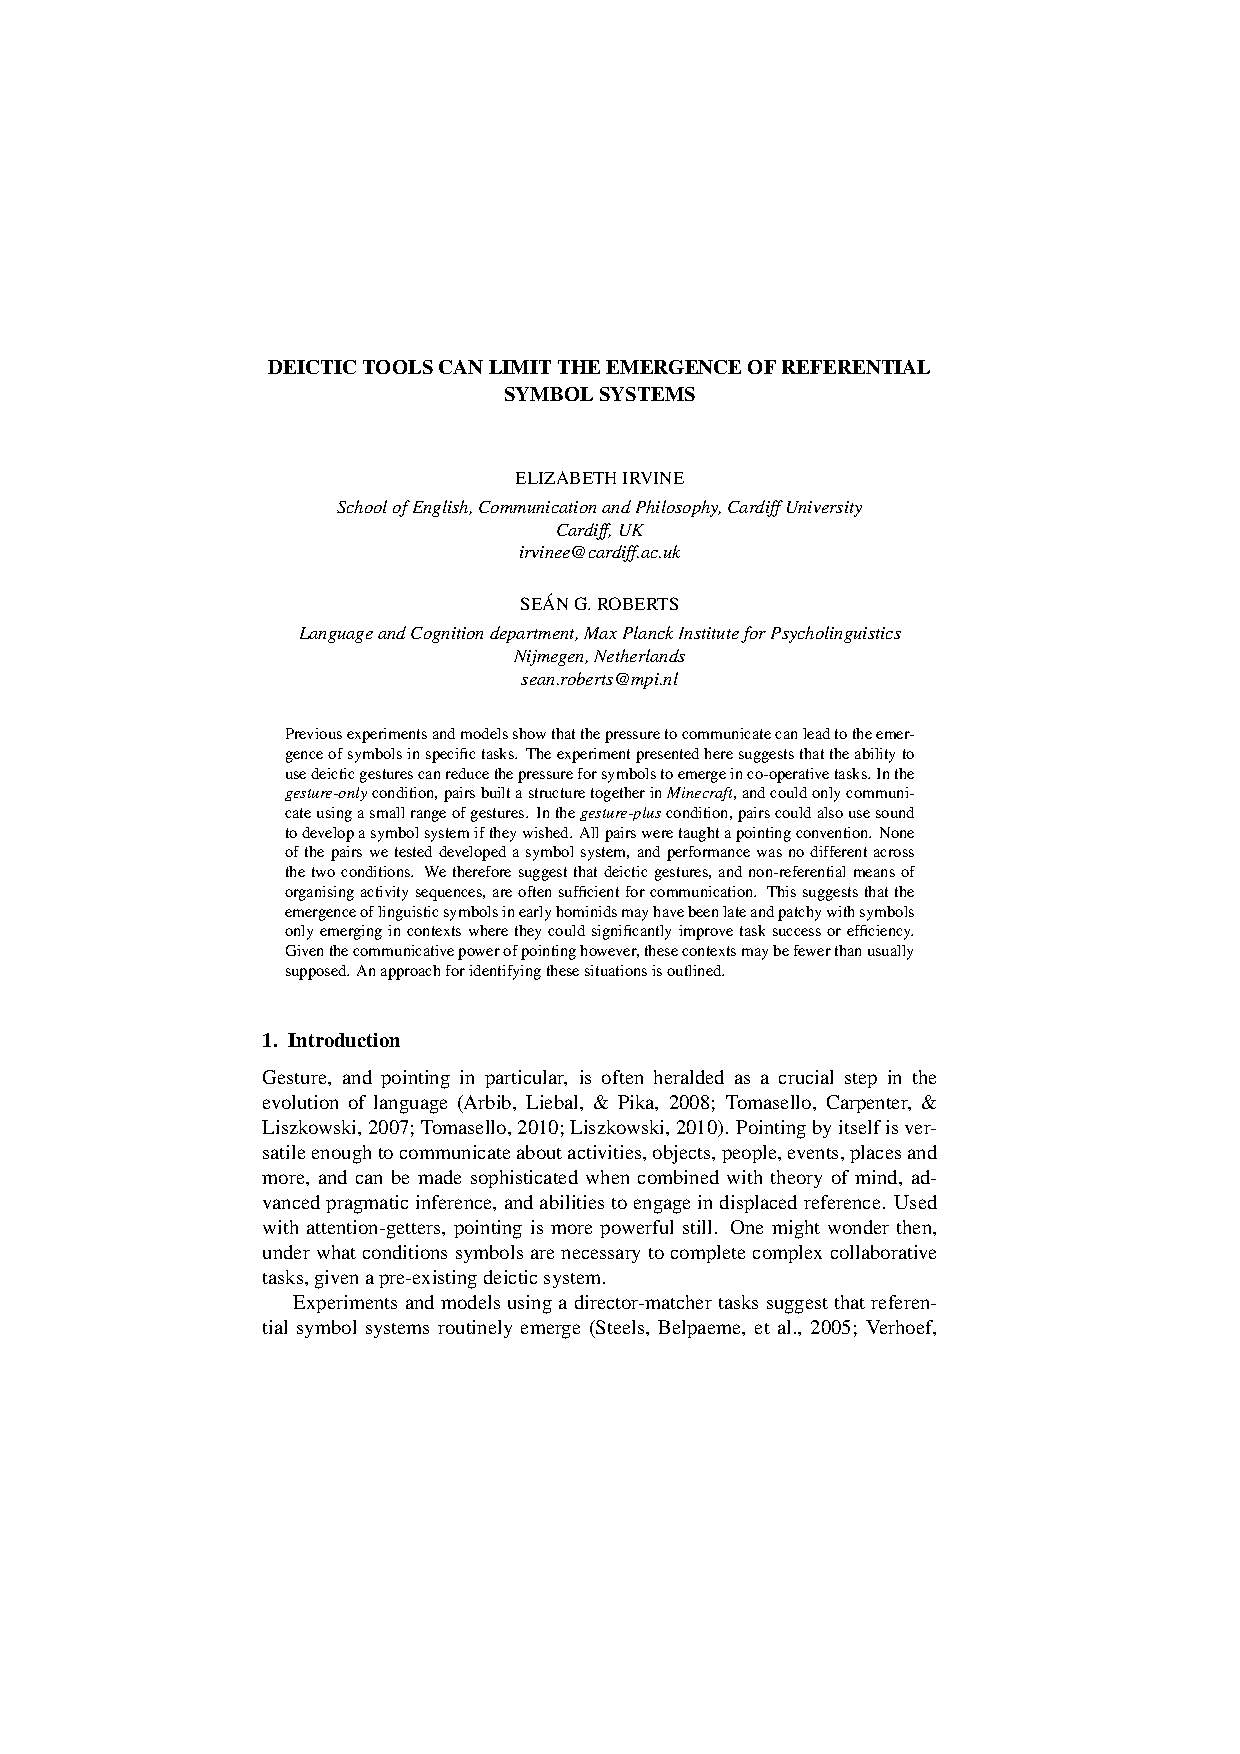
\includepdf[height=271.76470588235293mm, pages=-,pagecommand=\thispagestyle{plain}]{pdf/EVOLANG_11_paper_99.pdf}

\cleardoublepage




\index{Progovac Ljiljana}

\phantomsection
\label{paperp1}
\addcontentsline{toc}{chapter}{What Kind Of Grammar Did Early Humans (and Neanderthals) Command? A Linguistic Reconstruction, \newline \textit{ Ljiljana Progovac}}

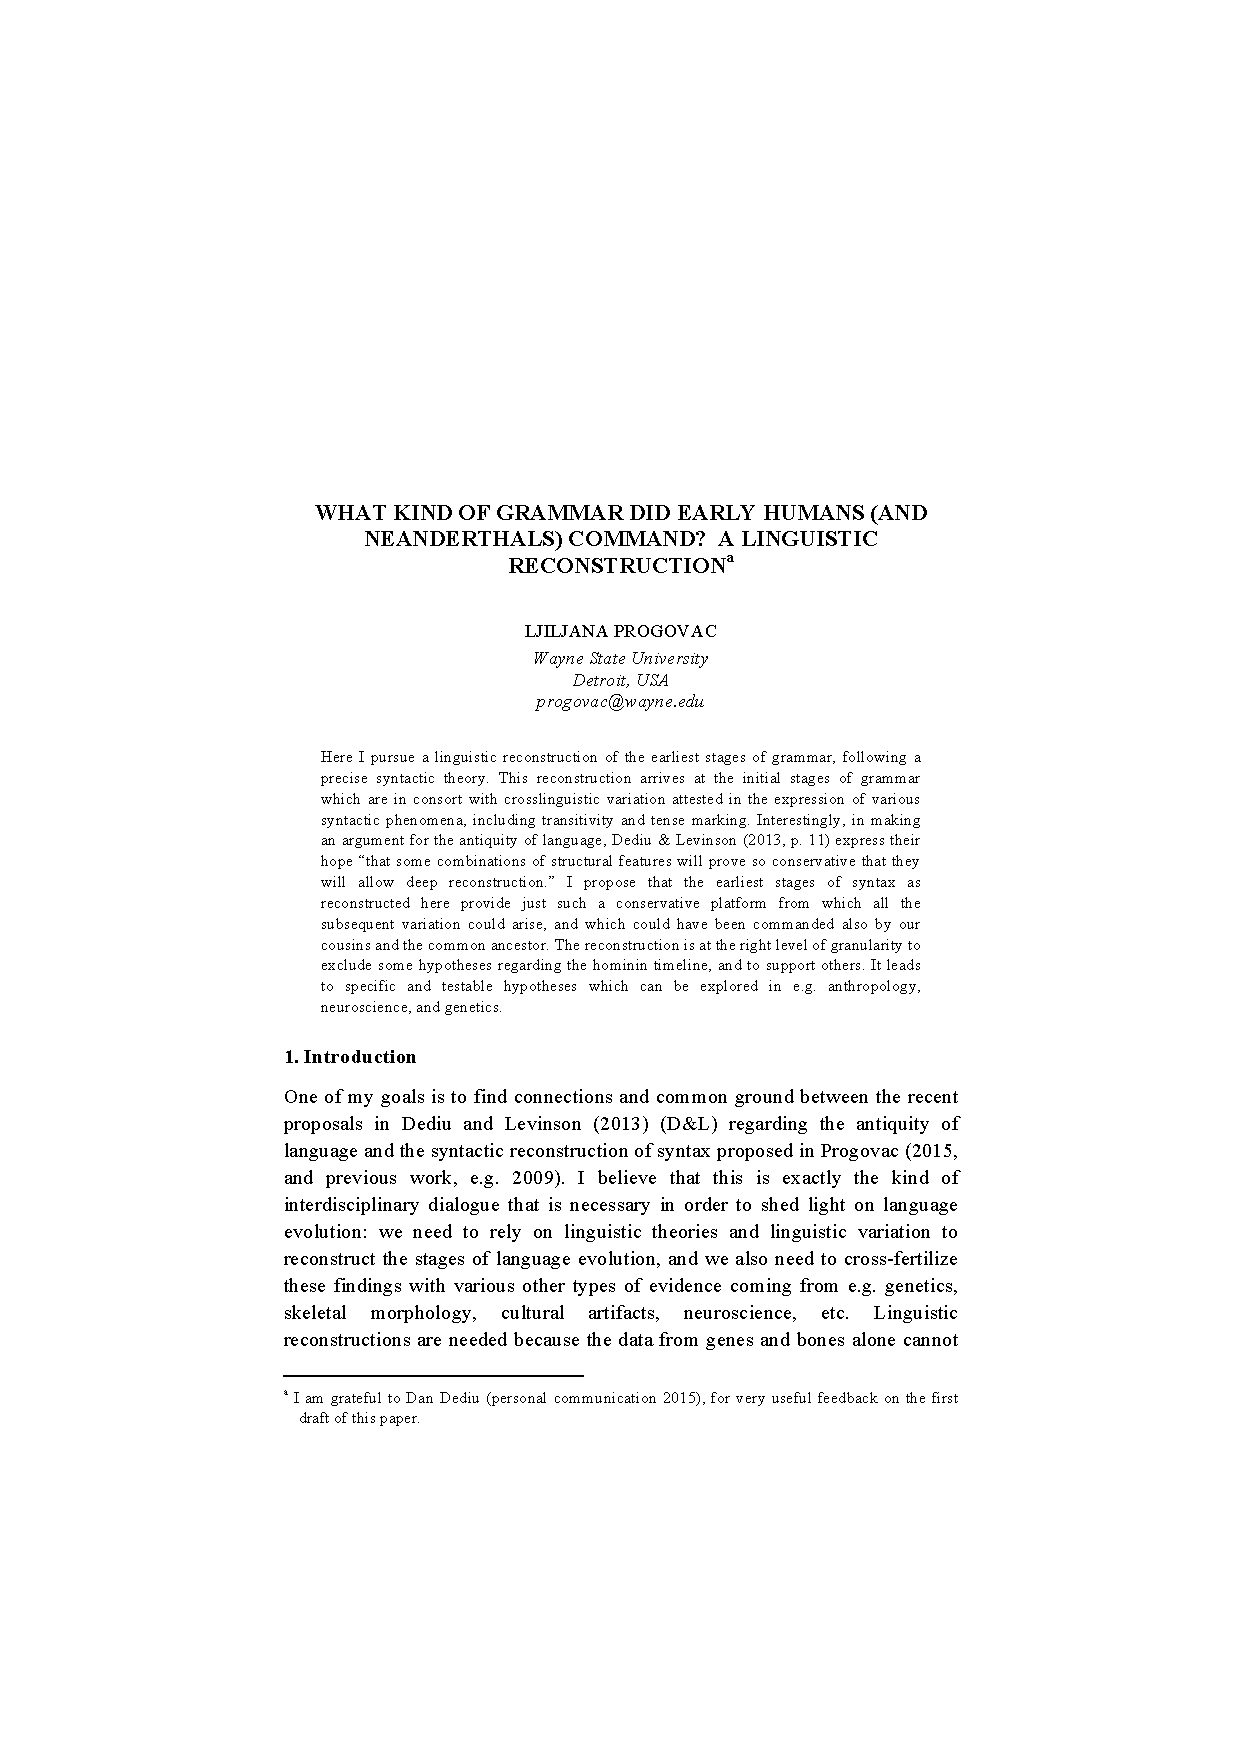
\includepdf[height=271.76470588235293mm, pages=-,pagecommand=\thispagestyle{plain}]{pdf/EVOLANG_11_paper_p1.pdf}

\cleardoublepage



\chapter*{Abstracts}
\addcontentsline{toc}{chapter}{\textbf{Abstracts}}
\cleardoublepage

\index{Janssen Rick}
\index{Winter Bodo}
\index{Dediu Dan}
\index{Moisik Scott}
\index{Roberts Sean}

\phantomsection
\label{paper86}
\addcontentsline{toc}{chapter}{Nonlinear Biases In Articulation Constrain The Design Space Of Language, \newline \textit{ Rick Janssen, Bodo Winter, Dan Dediu, Scott Moisik, Sean Roberts}}

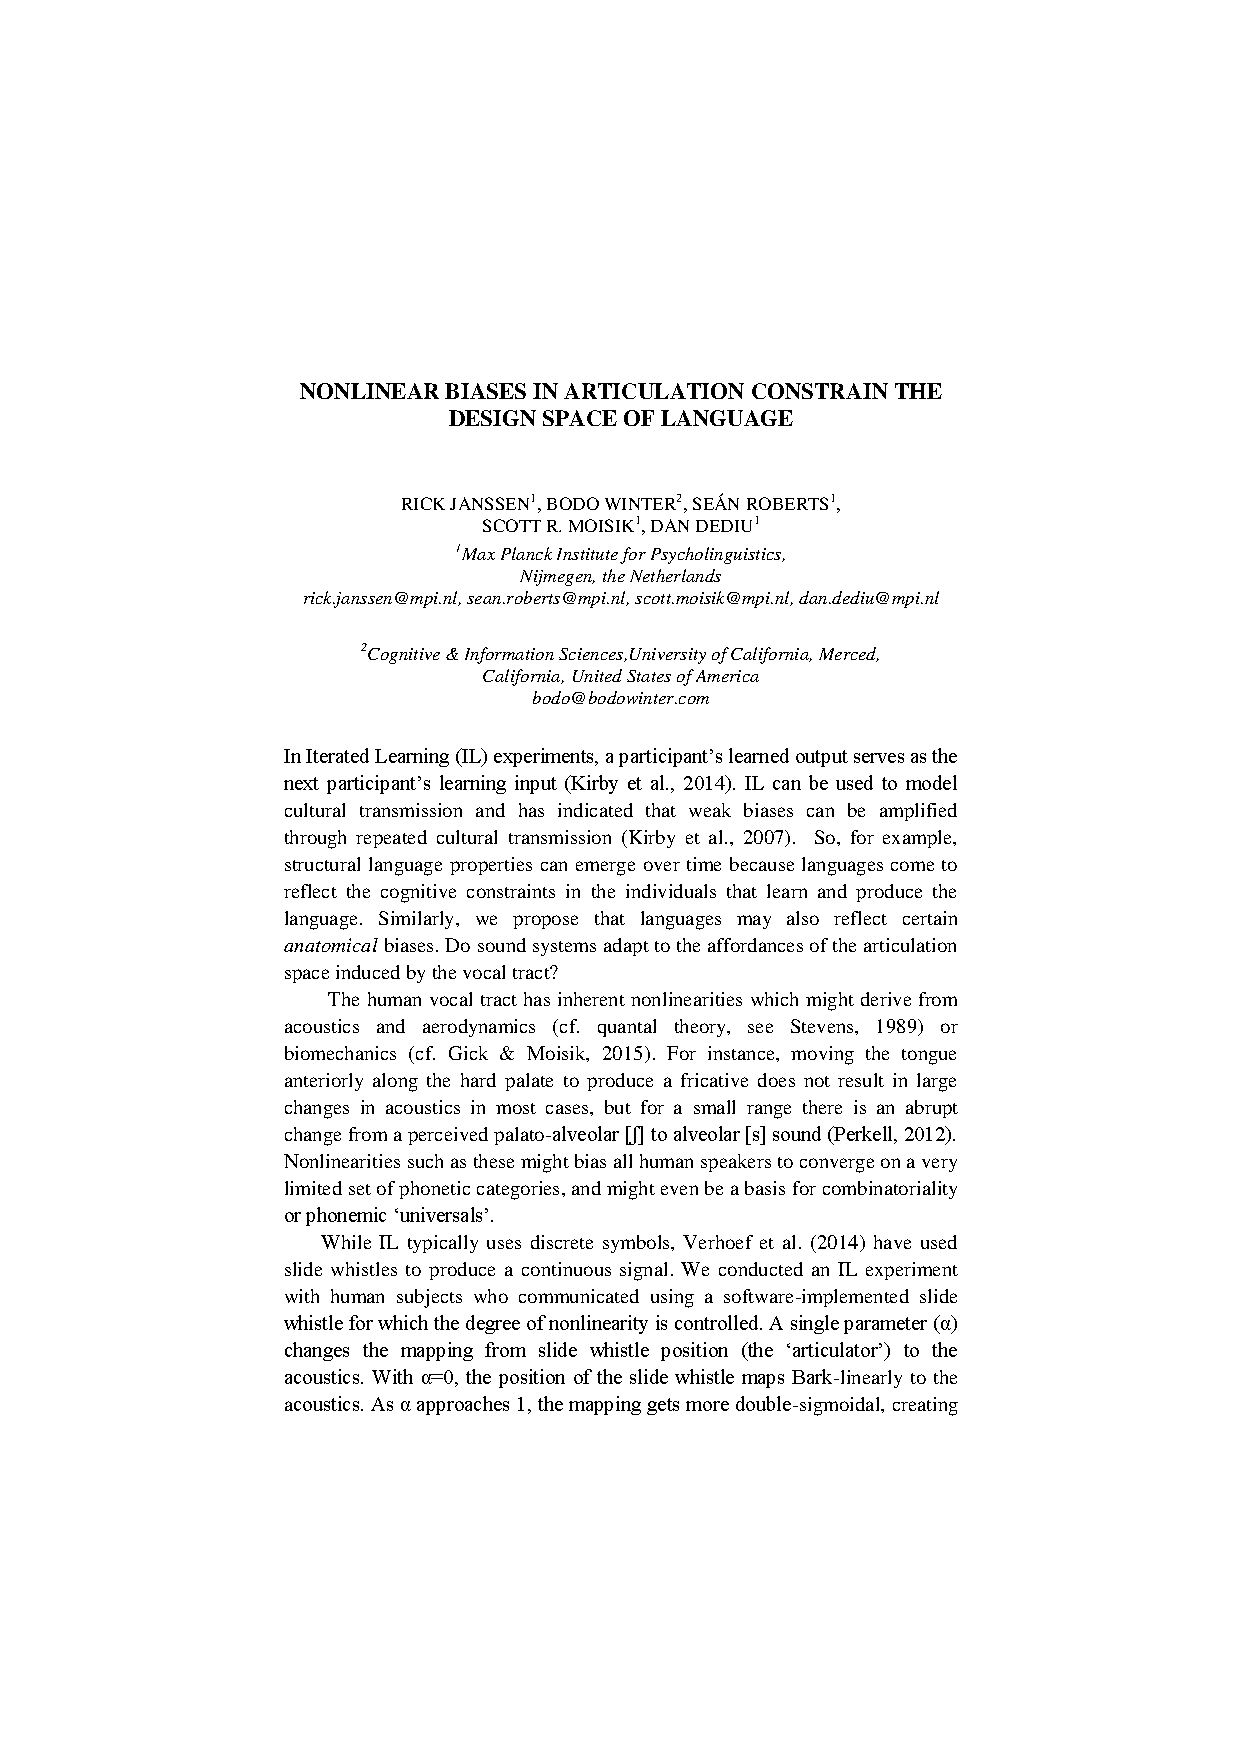
\includepdf[height=271.76470588235293mm, pages=-,pagecommand=\thispagestyle{plain}]{pdf/EVOLANG_11_paper_86.pdf}

\cleardoublepage



% Print the index of authors

\addcontentsline{toc}{chapter}{Index of authors}
\pagestyle{plain}
\printindex

\end{document}
